\chapter{Results and Discussion} \label{chap_results}

This chapter will present the results from performance testing our purposed architecture. Section \ref{sec_results} will present the setup to our experiments and their respective results, while Section \ref{sec_discussion} will provide our analysis of the results. 

%\section{Results} \label{sec_results}

\section{Hardware Resources}

As mentioned in Section \ref{sec_zedboard} we used a Zedboard, with an Artix-7 FPGa, for prototyping our suggested architecture. A short overview of the most vital resources available on the Artix-7 can be seen in Table \ref{tab_available_resources}. Table \ref{tab_resource_usage} shows the resource consumption of each accelerator as the number of accelerators increases. The "DSPs: Convoluter" column shows how many DSPs the covoluter module within the accelerator consumes.

As we can see from Table \ref{tab_resource_usage} the convoluter makes heavy usage of the DSPs. In its current state it contains $ 5 \times 5 $ MAC units, which optimally consumes four DSPs each. When the number of available DSPs is reduced, the MAC units need to exchange the DSP with LUTs, which causes an massive spike in resource consumption.

Since the accelerators optimal number of DSPs is 116 out the of 220 available, increasing the number of accelerators from one to two does not cause any critical spike in resource consumption. But the converting of 12 DSPs to LUT logic is still sigificant, causing a total of 4000 more LUTs being used. It reaches critical levels when we increases the number of accelerators to three, leaving only 50 DSPs to be used by each convoluter. This causes each accelerator to consume 18699 LUTs, giving a total of 56097, which exceeds the maximum of available LUTs by 2897. Thereby limiting the number of accelerators to two, unless we change to a larger FPGA.

This is unfortunate, since we would preferablly wish to run at least four accelerators in parallel, in order to exploit the bandwidth from all four high-performance AXI ports. We have been unable to explore ways to reduce the convoluters consumption of DSPs due to time constraints, but it is definitely something that should be done in future work. 

\begin{table}
	\centering
    \begin{tabular}{| >{\centering\arraybackslash}m{0.7in} |  >{\centering\arraybackslash}m{0.7in} |  >{\centering\arraybackslash}m{0.7in} |  >{\centering\arraybackslash}m{0.7in} |  >{\centering\arraybackslash}m{0.7in} |} 
    \hline
    Nof. accelerators & Slice LUTs & Flip-flops & DSPs & DSPs: Convoluter \\ \hline
    1 & 7986 & 3310 & 116 & 100 \\ \hline
    2 & 9941 & 3310 & 110 & 94 \\ \hline
    3 & 18699 & 3310 & 66 & 50 \\ \hline
    4 & 20971 & 3325 & 54 & 50 \\ \hline
        \end{tabular}
    \caption{Table showing how the resource usage varies for each accelerator as the number of accelerators increases.}
   	\label{tab_resource_usage}
\end{table}


\begin{table}
	\centering
    \begin{tabular}{| >{\centering\arraybackslash}m{1.0in} |  >{\centering\arraybackslash}m{1.0in} |  >{\centering\arraybackslash}m{1.0in} |} 
    \hline
    Slice LUTs & 53,200   \\ \hline
    Flip-flops & 106,400 \\ \hline
    DSPs & 220 \\ \hline
        \end{tabular}
    \caption{Available resources on the Artix-7 FPGA}
   	\label{tab_available resources}
\end{table}


\section{Performance}

\subsection{Setup}

In order to determine the execution speed and power efficiency of our system we have compared it to the ARM Cortex-A9 CPU on the Zedboard and an ASUS X550JK laptop with a Intel Core i7 4710HQ CPU. Both CPUs ran the pure software implementation of the CNN, while our system used a combination of hardware and software, as described in \ref{chap_method}. We ran our own system with three different configurations:

\begin{itemize}
\item Acc: 1 layer: Accelerating C1 and S2.
\item Acc: 2 layers: Accelerating C1, S2, C3 and S4.
\item Acc: 3 layers: Acceleraating C1, S2, C3, S4 and C5.
\item 2 Acc: 2 layers: Running to accelerators in parallel, on layer C1, S2, C3 and S4.
\end{itemize}

In order to determine the energy efficiency of the different systems we used the metric \textit{images/Watt}, i.e. number of images processed per Watt. We also included a metric for measuring execution speed, using images/second. Despite power efficiency being the main focus of this assignment, execution speed can be interesting for several applications and is closely related to power usage. Note that these images are $ 32 \times 32 $, and thus processing one image corresponds to 331104 multiply-and-accumulate operations. Thus, if one wish to convert the metric images/second to operations/second, one simply need to multiply with that number.

The measurements were done by timing the processing of 10 000 images from the MNIST dataset, while measuring the power consumption. 

Total board power was determined by measuring the voltage over pin 1 and 2 on J21 current sense resistor on the Zedboard during execution. We can then use the following equation to calculate the power consumption:

\begin{equation}\label{eq_power_measurement}
 P = (V_{in}-V_{measured}) \times \frac{V_{measured}}{R}
\end{equation}

Where $ V_{in} $ is the input voltage 12V, $ V_{measured} $ is the measured voltage across the pins, which have a resistance of $ R = 10m\Omega $.

With the FPGA programmed and the accelerator activated the board measured to 4.18 W, while the ARM processor alone measured to 3.82 W. The second core was turned off in both cases. We were unable to measure the power consumption of the laptop directly, and therefore used the power estimation provided by ASUS \cite{ASUS2015}. The laptop CPU uses 47 W, and including RAM, motherboard and various peripherals, we estimate a total consumption of 60W. Do note that this estimate is not completely accurate, and could potentially be lower. 


\subsection{Discussion} \label{sec_result_discussion}

\begin{figure}[h!]
	\centering
	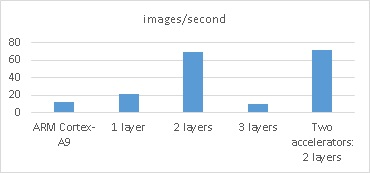
\includegraphics[width=1.0\textwidth]{Figures/Results/results_acc_improvements}
	\caption{Overview of how the performance changes with different configurations of the system.}
	\label{fig_results_acc_improvements}
\end{figure}

Figure \ref{fig_results_acc_improvements} shows how processing the different layers in hardware affect the performance. We can see that accelerating one layer provides us with a minor speedup, while accelerating two layers give almost 6x speedup. In stark contrast, accelerating C5 slows down the system and performs even worse than the ARM processor. We believe this is mainly due to how we move data to the accelerator. Each of the 120 outputs from C5 are computed using the same 16 input maps, but with a different set of 16 different kernels. This means that in the current state of our system we transfer the same 16 input maps 120 times to the accelerator. Which can be considered an rather ieffective use of bandwidth. A better memory scheme is discussed in Chapter \ref{chap_future_work}.

Another interesting aspect of Figure \ref{fig_results_acc_improvements} is that adding another accelerator, when two layers are accelerated, provides virtually no speedup. We have to primary explainations for this: 1) the accelerator starves, i.e. not fed data fast enough, and 2) the main bottleneck in now C5, which reduces the significance of improving performance for the previous layers.

Figure \ref{fig_performance_C1C2_only_accs} supports these explainations to a degree. The figure shows the performance of only processing layer C1, S2, C3 and S4. This shows that C5/F6 stands for 75\% of the processing time of the whole network. Since C5 48120 connections and F6 has 120, it is clear that C5 is the main bottleneck. These results is what caused us to a hot-fix of our system, so C5 could use our accelerator. But the previous figure gives a clear indication that the extension needs to be implemented more sophistically.

\begin{figure}[h!]
	\centering
	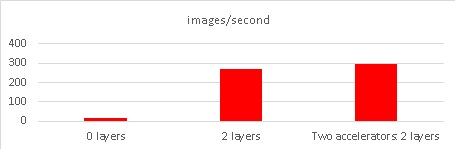
\includegraphics[width=1.0\textwidth]{Figures/Results/performance_C1C2_only_accs}
	\caption{Performance when only executing layer C1, S2, C3 and C4.}
	\label{fig_performance_C1C2_only_accs}
\end{figure}

While Figure \ref{fig_performance_C1C2_only_accs} shows where the major bottleneck is, it does not explain why adding another accelerator provides only a minor speedup. In turns out that the DMA bug (see Section \ref{sec_hardware_driver}, which forces us to re-initialize the DMA after it is done processing a BD ring, is part of the explaination. This re-initialiation causes the memory needed to store the BD rings for the DMA channels to be reallocated every time, and this takes time. In order to predict the performance if this bug was fixed, we measured the time it took re-initialize the DMA and subtracted it from the execution time.

\begin{figure}[h!]
	\centering
	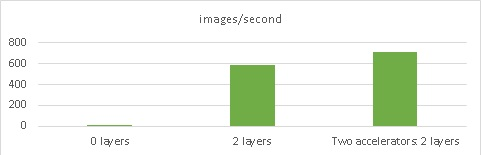
\includegraphics[width=1.0\textwidth,height=5cm]{Figures/Results/performance_sub_dma_init}
	\caption{Performance when only executing layer C1, S2, C3 and C4, and substracting DMA initializations.}
	\label{fig_performance_sub_dma_init}
\end{figure}

This produced the results seen in Figure \ref{fig_performance_sub_init}. We can see that this increases the performance  by more than 2x, and brings the configuration using two accelerators closer to being twice as fast as the one using one accelerator. But we can still see that there is something that is preventing the system to fully exploit having two accelerators running in parallel. We suggest two probable reasons for this:

\begin{enumerate}
\item Currently the processor has to wait for the data transfers to and from the accelerator to finish, without doing anything productively. This causes the accelerators to be starved, since the processors have to set up the transfers while the accelerators do not have to data to consume. Preferably it could set up the other transfers while the accelerator is processing and/or the DMA performes transfers, but due to the initialization bug we have been unable to implement this. 
\item Another fault of the design is that the input buffer to the accelerator has to be filled before it can start processing. A better soultion would be to simply stream the data into the accelerator, and make stall when data is not available. 
\end{enumerate}


\begin{figure}[h!]
	\centering
	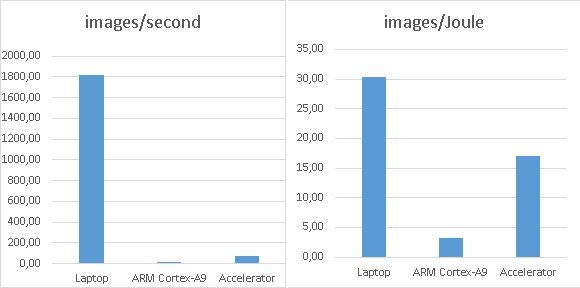
\includegraphics[width=1.0\textwidth,height=5cm]{Figures/Results/performance_whole_system}
	\caption{Performance when computing the whole network.}
	\label{fig_performance_whole_system}
\end{figure}

\begin{figure}[h!]
	\centering
	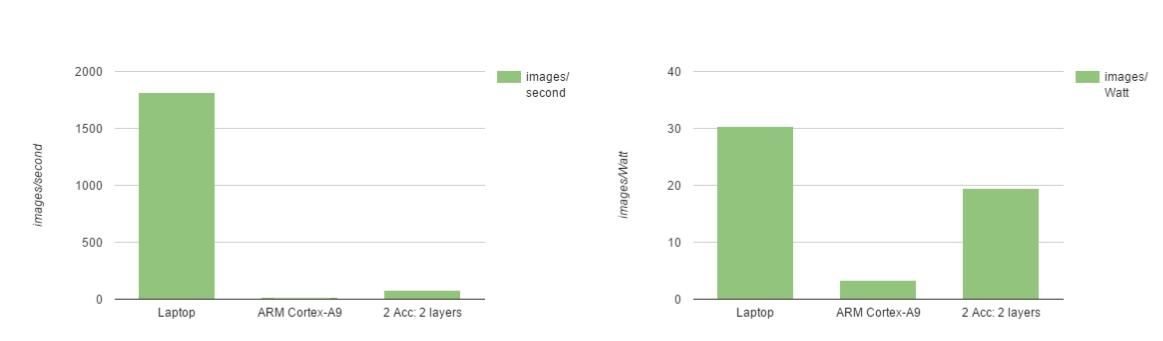
\includegraphics[width=1.0\textwidth,height=5cm]{Figures/Results/performance_whole_system_sub_dma_init}
	\caption{Performance when computing the whole network, but subtracts the DMA initializations.}
	\label{fig_performance_whole_system_sub_dma_init}
\end{figure}

In Figure \ref{fig_performance_whole_system} we can see how our system performs compared to the laptop CPU. In the current state of the system it gets handely outperformed by the laptop, even if we subtract the DMA initializations (Figure \ref{fig_performance_whole_system_sub_dma_init}. The primary reason for this is the bottleneck created by C5. If we look at the performance when considering only layer C1, S2, S3 and C4 our system is 2x as energy efficient, as seen in Figure \ref{fig_performance_C1C2_laptop}. And Figure \ref{fig_performance_C1C2_laptop_sub_dma_init} shows it is almost 5x as power efficienct if we assume the DMA initialization bug gets fixed. 

\begin{figure}[h!]
	\centering
	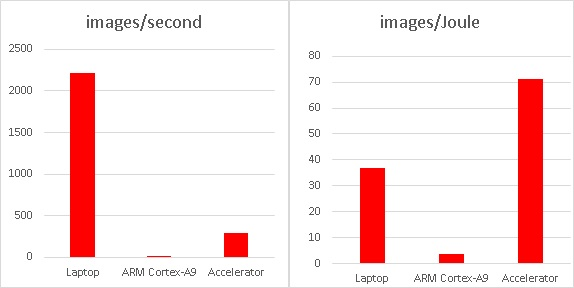
\includegraphics[width=1.0\textwidth,height=5cm]{Figures/Results/performance_C1C2_laptop}
	\caption{Performance when only processing C1, S2, C3 and S4.}
	\label{fig_performance_C1C2_laptop}
\end{figure}

\begin{figure}[h!]
	\centering
	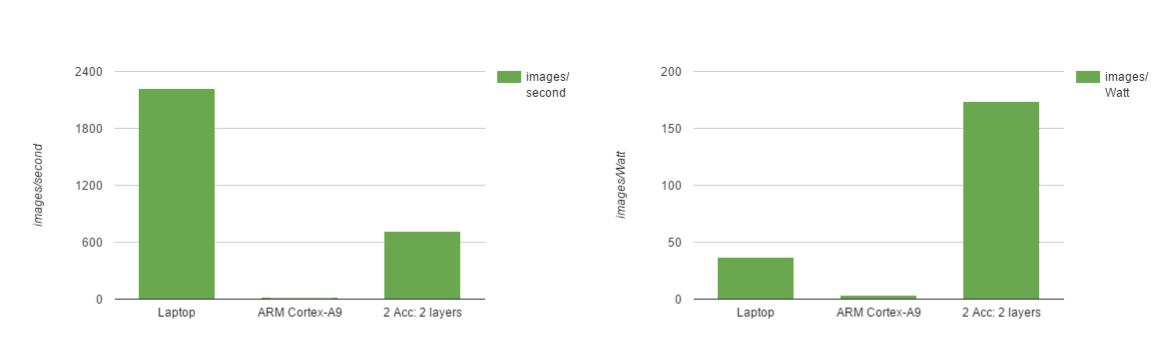
\includegraphics[width=1.0\textwidth,height=5cm]{Figures/Results/performance_C1C2_laptop_sub_dma_init}
	\caption{Performance when only processing C1, S2, C3 and S4, but assuming that the DMA initialization bug is fixed.}
	\label{fig_performance_C1C2_laptop_sub_dma_init}
\end{figure}

It is worth noticing that our system is currently only a prototype, and there remains several performance boosting features and optimizations that can be implemented. We have dedicated Chapter \ref{chap_future_work} for this discussion. 
